\documentclass{beamer}
\usepackage{../common_slides}


\title{Text Classification\\ + \\ Machine Learning Review 2 }
\date{}
\author{CS 287}
\begin{document}


\begin{frame}
  \titlepage
\end{frame}

j

\begin{frame}{Quiz: Naive Bayes}
  Given bag-of-word features \[\mcF = \{\mathrm{\texttt{The, movie, was, terrible, rocked, A}} \}\] and two training data points:

  \begin{center}
    Class 1: \texttt{The movie was terrible}

    Class 2: \texttt{The movie rocked}
  \end{center}
  \\

  \air

  What is the conditional distribution $P(Y | X)$ of the new example ``\texttt{terrible movie}''  with $\alpha =0$?
  \air

  What about ``\texttt{A terrible movie}'' with $\alpha =1$ ?
\end{frame}

\begin{frame}{Answer: Naive Bayes (1) }
  \texttt{terrible movie}
  \air

  Prior is simple: $p(\boldy) =  \begin{bmatrix} 1/2 & 1/2 \end{bmatrix}$

  Construct count matrix:
  \[ \boldF =
    \begin{bmatrix}
      1 & 1 & 1 & 1 & 0 & 0 \\
      1 & 1 & 0 & 0 & 1 & 0 \\
    \end{bmatrix}
  \]

  With $\alpha = \epsilon$,

  \[ p(\boldx | \boldy) =     \begin{bmatrix}
      1/4 & 1/4 & 1/4 & 1/4 & 0 & 0 \\
      1/3 & 1/3 & 0 & 0 & 1/3 & 0 \\
    \end{bmatrix}
  \]

  \[ p(\boldy | \boldx) \propto \begin{bmatrix} 1/2 \times 1/2 \times 1/2 &  1/2 \times 0 \times 1/3  \end{bmatrix} = \begin{bmatrix} 1 &  0 \end{bmatrix}  \]

\end{frame}

\begin{frame}{Answer: Naive Bayes (2) }
  \texttt{A terrible movie}
  \air

  With $\alpha = 1$,

  \[ \bar{\boldF} =
    \begin{bmatrix}
      2 & 2 & 2 & 2 & 1 & 1 \\
      2 & 2 & 1 & 1 & 2 & 1 \\
    \end{bmatrix}
  \]

  \[ p(\boldx | \boldy) =     \begin{bmatrix}
      1/5 & 1/5 & 1/5 & 1/5 & 1/10 & 1/10 \\
      2/9 & 2/9 & 1/9 & 1/9 & 2/9 & 1/9 \\
    \end{bmatrix}
  \]

  \begin{eqnarray*}
    p(\boldy | \boldx) &\propto& \begin{bmatrix} 1/2 \times 1/10 \times 1/5 \times 1/5 &  1/2 \times 1/9 \times 1/9 \times 2/9  \end{bmatrix} \\
    &\approx&     \begin{bmatrix} 0.593 & 0.407 \end{bmatrix}
  \end{eqnarray*}



\end{frame}
\section{Classification Review}

\begin{frame}{Review: Multiclass Sentiment}
    \begin{itemize}
    \item
      $\star \star \star \star$

      I visited The Abbey on several occasions on a visit to Cambridge and found it to be a solid, reliable and friendly place for a meal.

    \item $\star \star$

      However, the food leaves something to be desired. A very obvious menu and average execution

    \item $\star \star \star \star \star$

      Fun, friendly neighborhood bar. Good drinks, good food, not too pricey. Great atmosphere!
  \end{itemize}
\end{frame}



\begin{frame}{Review: Sparse Bag-of-Words Features}
  Representation is counts of input words,
  \begin{itemize}
  \item $\mcF$; the vocabulary of the language.
  \item $\boldx = \sum_{i} \bolddelta(f_i)$
  \end{itemize}

  Example: Movie review input,
  \begin{center}
    \texttt{A sentimental mess}
    \[ \boldx = \bolddelta(\texttt{word:A}) + \bolddelta(\texttt{word:sentimental}) +
    \bolddelta(\texttt{word:mess}) \]
    \[ \boldx^\top =\begin{bmatrix} 1 \\ \vdots
        \\ 0\\ 0 \\ \end{bmatrix} +\begin{bmatrix} 0 \\
        \vdots \\ 0\\ 1 \\ \end{bmatrix} +
     \begin{bmatrix} 0 \\ \vdots \\ 1\\ 0 \\ \end{bmatrix}
    =\begin{bmatrix} 1 \\ \vdots \\ 1 \\ 1 \\ \end{bmatrix}
    \begin{matrix*}[l] \mathrm{\texttt{word:A}} \\ \vdots \\ \mathrm{\texttt{word:mess}} \\ \mathrm{\texttt{word:sentimental}} \\ \end{matrix*}
     \]
  \end{center}
\end{frame}



\begin{frame}{Review: Output Class Notation}
  \begin{itemize}
  \item $\mcC = \{1, \ldots, \dout\}$; possible output classes
  \item $c \in \mcC$; always one true output class
  \item $\boldy = \bolddelta(c) \in \reals^{1\times \din}$; true one-hot output representation

  % \item Note: when classes are words, we call them \textit{word types}.
  \end{itemize}
\end{frame}

\begin{frame}{Review: Multiclass Classification}
  Examples: Yelp stars, etc.
  \begin{itemize}
  \item $\dout = 5$; for examples
  \item In our notation, one star, two star...
    \begin{eqnarray*}
      \star \ c = 1 & \  \boldy &= \begin{bmatrix} 1 & 0 & 0 & 0 & 0  \end{bmatrix}  \mathrm {\ vs. \ } \\
    \star \star \ c = 2 & \boldy &=    \begin{bmatrix} 0 & 1 & 0 & 0 & 0 \end{bmatrix} \ldots
   \end{eqnarray*}
  \end{itemize}
  Examples: Word Prediction (Unit 3)
  \begin{itemize}
  \item $\dout > 100,000$;
  \item In our notation, $\mcC$ is vocabulary and each $c$ is a word.
    \begin{eqnarray*}
      the \ c = 1 & \  \boldy &= \begin{bmatrix} 1 & 0 & 0 & 0 & \ldots & 0  \end{bmatrix}  \mathrm {\ vs. \ } \\
      dog \ c = 2 & \boldy &=    \begin{bmatrix} 0 & 1 & 0 & 0 & \ldots & 0 \end{bmatrix} \ldots
   \end{eqnarray*}
  \end{itemize}
\end{frame}


\begin{frame}{Review Linear Models for Classification}
  Linear model,
  \[\hat{\boldy} = f(\boldx \boldW + \boldb)\]
  \begin{itemize}
  \item $\boldW \in \reals^{\din \times \dout}, \boldb \in \reals^{1 \times \dout}$; model parameters
  \item $f: \reals^{\dout} \mapsto \reals^{\dout}$; activation function
  \item Sometimes $\boldz = \boldx \boldW + \boldb$ informally ``score'' vector.
  \item Note $\boldz$ and $\hat{\boldy}$ are not one-hot.
  \end{itemize}

  \air

  Class prediction,
  \[ \hat{c} = \argmax_{i \in \mcC} \hat{y_i}  = \argmax_{i \in \mcC} (\boldx \boldW + \boldb)_i    \]
\end{frame}


\begin{frame}{Probabilistic Linear Models}
  % Estimate
  Can estimate a linear model probabilistically,

  \begin{itemize}
  \item Let output be a random variable $Y$, with sample space $\mcC$.
  \item Representation be a random vector $X$.
  \item (Simplified frequentist representation)
  \item Interested in estimating parameters $\theta$,
      \[ P(Y | X; \theta) \]
  \end{itemize}
  Informally we use $p(\boldy=\bolddelta(c) | \boldx)$ for
  $P(Y = c | X = \boldx)$.

\end{frame}

\section{Discriminative Models}

\begin{frame}{Discriminative Model. Conditional Log-Likelihood as Loss }
  % Estimate
  \begin{itemize}
  \item $(\boldx_1, \boldy_1), \ldots, (\boldx_n, \boldy_n)$; supervised data
  \item Parameters maximize conditional likelihood of training data.
    \[ \mathcal{L}(\theta) =  - \sum_{i=1}^n \log p(\boldy_i | \boldx_i ; \theta) \]
  For linear models $\theta = (\boldW, \boldb)$
   \item (Contrast with generative models like NB, $p(\boldx_i, \boldy_i)$ )
  \item Do this by minimizing negative log-likelihood (NLL).
    \[ \argmin_\theta \mathcal{L}(\theta)\]
  \end{itemize}
\end{frame}


\begin{frame}{The Softmax}

  Alternative parametrization of probabilistic model.


  Use a softmax to force a distribution,

  \[\softmax(\boldz) = \frac{\exp(\boldz)}{\displaystyle \sum_{c } \exp(z_c)}  \]

  \[\log \softmax(\boldz) = \boldz - \log \sum_{c} \exp(z_c)  \]


  \begin{itemize}
  \item Exercise: Confirm always gives a distribution.

  \item Denominator known as \textit{partition} function (we'll see many times).
  \end{itemize}

\end{frame}



\begin{frame}{Why is it called the softmax?}

  \begin{columns}[t]
    \begin{column}[t]{0.5\textwidth}


      \begin{figure}
        \centering
        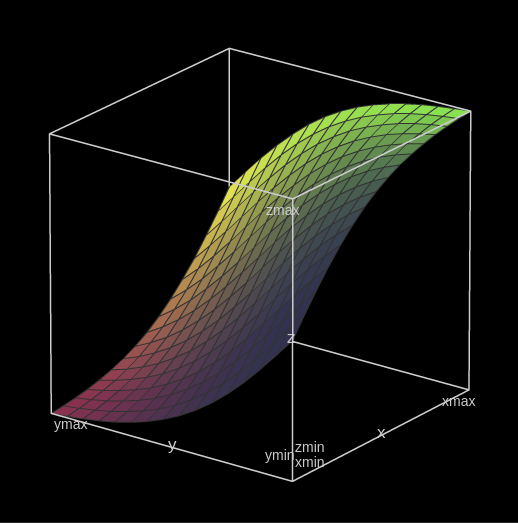
\includegraphics[width=5cm]{softmax}
      \end{figure}
      \[\softmax([x\ y]) = \frac{\exp(x)}{\displaystyle  \exp(x) + \exp(y)}  \]
    \end{column}

    \begin{column}[t]{0.5\textwidth}


      \begin{figure}
        \centering
      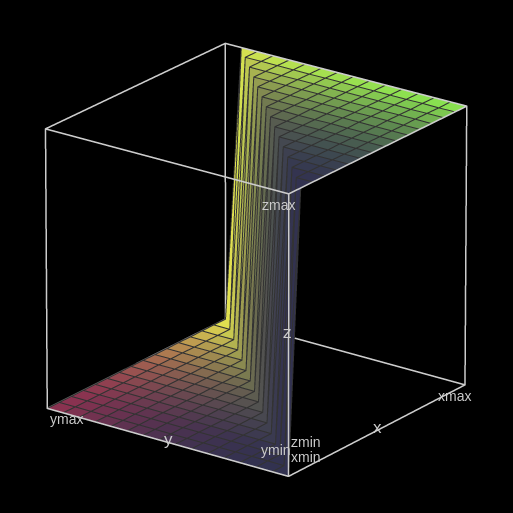
\includegraphics[width=5cm]{argmax}
      \end{figure}
      \[\argmax([x\ y]) = \indicator(x > y) \]
    \end{column}
  \end{columns}
\end{frame}

\begin{frame}{Multiclass Logistic Regression}
  \begin{itemize}
  \item Direct estimation of conditional $p(\boldy =c | \boldx; \theta)$

    \[\hat{\boldy} =  p(\boldy =c | \boldx; \theta) =  \softmax(\boldx \boldW + \boldb) \]
  \item $\boldW \in \reals^{\din \times \dout}, \boldb \in \reals^{1 \times \dout}$; model parameters

  \item ``Regression'' of the distribution.
  \item Classification still done as,
    \[ \hat{c} =  \argmax_{c \in \mcC} (\boldx \boldW + \boldb)_c  \]

  \end{itemize}

  % Directly estimate the conditional distribution.


  %   \[ \log p(\boldy =c | \boldx; \theta) = \hat{y} = \log \softmax(\boldz) =
  %     \frac{\exp(z_c)}{ \sum_{\displaystyle c'} \exp(z_{c'})}   \]
  %   \begin{itemize}


  %   \end{itemize}
  % \[ \hat{\boldy} = f(\boldx \boldW + \boldb) \]
\end{frame}

\begin{frame}{Example: Multiclass Logistic Regression}
  3 classes, 2 features,

  \begin{eqnarray*}
    \boldW = \begin{bmatrix} 1  & 2 & -1 \\ -8 & 2 & 3 \\ \end{bmatrix}  &&   \boldb = \begin{bmatrix} 0  & 0  & 0\\ \end{bmatrix} \ \  \boldx = \begin{bmatrix} 1  & 0 \\ \end{bmatrix} \\
  \end{eqnarray*}
  \[ \boldz = \boldx \boldW + \boldb = \begin{bmatrix} 1 & 2 & -1 \\ \end{bmatrix} \]

  Log-partition function,
  \[ \log \sum_c \exp(z_c) = \log ( \exp(1)  +  \exp(2) + \exp(-1) ) \approx 2.349 \]

  \[\log \softmax(\boldz) \approx \begin{bmatrix}  1 - 2.349   &  2- 2.349 & -1 - 2.349 \\ \end{bmatrix}  \]

  \[p(\boldy| \boldx) = \begin{bmatrix} 0.259 & 0.705 & 0.035 \end{bmatrix}   \]
\end{frame}

\begin{frame}{Important Case: Logistic Regression}
  For binary classification:
  \begin{eqnarray*}
   \softmax([z_1\ z_2]) &=& \frac{\exp(z_1)}{\exp(z_1) + \exp(z_2)} \\
 &=& \frac{1}{1 + \exp(-(z_1-z_2))} = \sigma(z_1 -z_2)
  \end{eqnarray*}

  Logistic sigmoid function:
  \[\sigma(t) = \frac{1}{1 + \exp(-t)} \]
  \begin{figure}
    \centering
    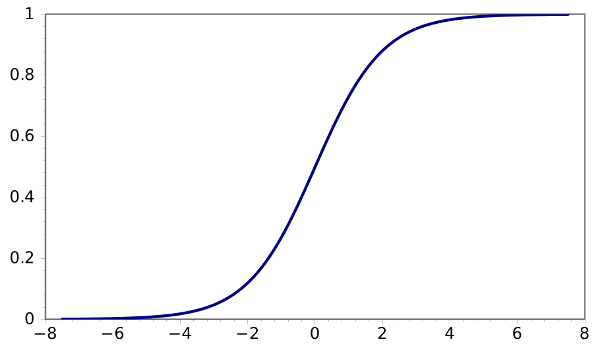
\includegraphics[width=5cm]{sigmoid}
  \end{figure}
\end{frame}

\begin{frame}{Multiclass Logistic Regression: A Model with Many Names}
  \begin{itemize}
  \item  Multinomial Logistic Regression


  \item Log-Linear Model (particularly in NLP)

    \[\log \softmax(\boldz) = \boldz - \log \sum_{c} \exp(z_c)  \]


  \item Softmax Regression


  \item Max-Entropy (MaxEnt)


  \end{itemize}
\end{frame}

\section{Loss}

\begin{frame}{Regression with Squared Loss }
  Define the squared error of two points $\boldp$ and $\boldq$,
  \[ \textrm{squared-error}(\boldp, \boldq)= ||\boldp - \boldq||^2_2  \]

  Can use to compare true with prediction,

  \[L_{squared-error}(\boldy, \hat{\boldy}) = ||\boldy - \hat{\boldy}||^2_2 \]

  Common case, when $y_c = 1$ for class $c$,
  \[L_{squared-error}(\boldy, \hat{\boldy}) = ||\bolddelta(c) - \hat{\boldy} ||_2^2  \mathrm{\ where\ }y_c = 1 \]

  \textbf{Not} a good metric for comparing distributions.
\end{frame}


\begin{frame}{Cross-Entropy Loss}
  Define the cross-entropy of two distributions $\boldp$ and $\boldq$,
  \[ H(\boldp, \boldq)= -\sum_{c}p_{c'} \log q_{c'}  \]

  Can use to compare true with prediction,

  \[L_{cross-entropy}(\boldy, \hat{\boldy}) = - \sum_{c} y_{c'} \log \hat{y}_{c'} \]

  Common case, when $y_c = 1$ for class $c$,
  \[L_{cross-entropy}(\boldy, \hat{\boldy}) = - \log \hat{y}_c \mathrm{\ where\ }y_c = 1 \]

  \[ \hat{\boldy} = p(\boldy_i | \boldx_i; \theta) \]
\end{frame}

\begin{frame}{Loss Minimization}
    \[ L_{cross-entropy}(\boldy, \hat{\boldy})=  - \log \hat{y}_c \mathrm{\ where\ }y_c = 1   \]

  Equivalent to probabilistic objective:

  \[ \mathcal{L}(\theta) =  - \sum_{i=1}^n \log p(\boldy_i | \boldx_i; \theta) = \sum_{i=1}^n L_{cross-entropy}(\boldy_i, \hat{\boldy}_i) \]


  And the distribution is parameterized as a softmax,
  \begin{eqnarray*}
    L_{cross-entropy}(\boldy, \hat{\boldy}) &=& - \log \hat{y}_c\\
    &=& -\log \softmax(\boldx \boldW + \bold b)_c \\
    &=& - z_c + \log \sum_{c' \in \mcC} \exp(z_{c'})
  \end{eqnarray*}

  However, this has \textbf{no closed form} for minimization.

\end{frame}

\begin{frame}{Objective}
  Complete objective:
  \[ \mathcal{L}(\theta) =  - \sum_{i=1}^n (\boldx_i \boldW + \boldb )_{c_i}  + \log \sum_{c'} \exp  (\boldx_i \boldW  + \boldb )_{c'} \]
  \begin{itemize}
  \item First term is linear in $\boldW$ (convex)
  \item Second term is log-sum-exp of a linear functions of $\boldW$ (convex).
  \item Objective is convex, but not strictly convex.
  \item Exercise(Hard) (Boyd and  Vandenberghe, 2004 p. 72-74)
  \end{itemize}
\end{frame}

\begin{frame}{Objective}
  \begin{figure}
    \centering
    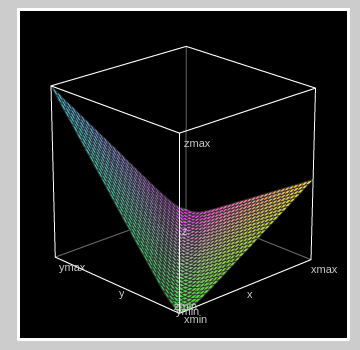
\includegraphics[width=5cm]{lrobj}
  \end{figure}

  \begin{center}
    Loss for 2 classes, only bias, parameters $x, y$
  \end{center}
  \[ L([x\ y]) = - 10 \log \softmax([x\ y])_1 -5\log \softmax([x\ y])_2 \]

\end{frame}

\begin{frame}{$\ell_2$ Regularization}

  \[ \mathcal{L}(\theta) = - \sum_{i=1}^n L(\boldy_i, \hat{\boldy}_i) + \frac{\lambda}{2} ||\theta||^2_2\]
  \begin{itemize}
  \item Prevents overfitting on the training data
  \item LR will naturally send $||W|| \rightarrow \infty$ (Murphy, p.252)
  \item Objective becomes strictly convex.
  \end{itemize}

\end{frame}


\begin{frame}{Regularized Optimization}
  \begin{figure}
    \centering
    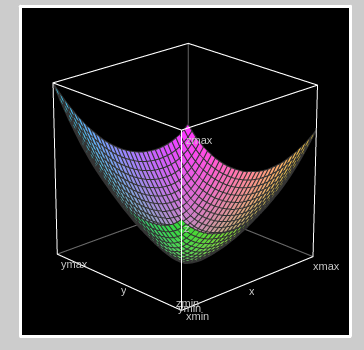
\includegraphics[width=5cm]{lrobjl2}
  \end{figure}

  \begin{center}
    Loss for 2 classes, only bias, parameters $x, y$, $\lambda=2$
  \end{center}
  \[ L([x\ y]) = - 10 \log \softmax([x\ y])_1 -5\log \softmax([x\ y])_2 + ||[x\ y]||_2^2\]

\end{frame}


\section{Optimization}
\begin{frame}{Review: Calculus!}
  \begin{align*}
    &\frac{d (w x)  }{d x} = w   & \frac{d (u/v) }{d x} = \frac{u'v -   uv'} {v^2}  \\
   &\frac{d \log u(x) }{d x} = \frac{u'}{u}  & \frac{d \exp u(x) }{d x} =  u' \exp u
  \end{align*}

  \begin{itemize}
  \item For function $f: \reals^n \mapsto \reals^m $ Jacobian is
    \[ \boldJ = \begin{bmatrix} \frac{\partial f(\boldx)_1}{\partial x_1} & \ldots&  \frac{\partial f(\boldx)_1}{\partial x_n} \\
      &\ddots& \\
      \frac{\partial f(\boldx)_m}{\partial x_1} & \ldots &  \frac{\partial f(\boldx)_m}{\partial x_n} \\
    \end{bmatrix}\]

     \item In-Class: Compute Jacobian of (1) $L$,  (2) $\softmax$, (3) $\boldz = \boldx \boldW + \boldb$
  \end{itemize}


\end{frame}


\begin{frame}{Symbolic Gradients}

  \begin{itemize}
  \item

  Partials of $L(\boldy, \hat{\boldy})$ for all $j \in \{1, \ldots, \dout\}$ and $y_c = 1$

  \[ \frac{\partial L(\boldy, \hat{\boldy})}{\partial \hat{y}_j} = \begin{cases}-\frac{1} {\hat{y}_j} & j = c\\ 0 & o.w. \end{cases}  \]
  \pause

  \item
    Partials of $\hat{\boldy} = \softmax(\boldz)$

  \[ \frac{\partial \hat{y}_j }{\partial z_i} =
    \begin{cases}
      \hat{y}_i (1 - \hat{y}_i) & i = j\\
      - \hat{y}_i \hat{y}_j & i \neq j \\
    \end{cases} \]

  \pause
  \item Partials of $\boldz  = \boldx \boldW + \boldb $

  \[ \frac{\partial z_i }{\partial b_{i'}} = \indicator(i = i') \ \  \frac{\partial z_i }{\partial W_{f, i'}} = x_f \indicator(i = i') \]

  \end{itemize}

\end{frame}

\begin{frame}{Review: Chain Rule}
  Assume we have a function and a loss:

  \[ f : \reals^n \rightarrow \reals^m \ \ \  L : \reals^m \rightarrow \reals \]

  Then for $i \in \{1, \ldots, n \}$

  \[ \frac{\partial L(f(\boldx))}{\partial x_i} = \sum_{j =1}^m \frac{\partial f(\boldx)_j} {\partial  x_i} \frac{\partial L(f(\boldx))} {\partial f(\boldx)_j}   \]


\end{frame}

\begin{frame}{Chain Rule}

  For multiclass logistic regression:

  \[ \frac{\partial L(\boldy, \hat{\boldy})}{\partial z_i} = \sum_{j} \frac{\partial \hat{y}_j }{\partial z_i}  \frac{\indicator(j = c)} {\hat{y}_j} =     \begin{cases}
      -(1 - \hat{y}_i) & i = c\\
      \hat{y}_i & ow. \\
    \end{cases} \]

  Therefore for parameters,

  \[\frac{\partial L}{\partial b_{i}} =
    \frac{\partial L}{\partial z_{i}} \ \ \ \ \frac{\partial L}{\partial W_{f, i}} =
     x_f \frac{\partial L}{\partial z_{i}}\]

   \pause
   Intuition:
   \begin{itemize}
   \item Nothing happens on correct classification.
   \item Weight of true features increases based on prob not given.
   \item Weight of false features decreases based on prob given.
   \end{itemize}
\end{frame}



\begin{frame}{Gradients-based minimization}
  Consider one example $(\boldx, \boldy)$, we compute ``forward'' and then ``backward'',

  \begin{enumerate}
  \item Compute scores $\boldz =  \boldx \boldW + \boldb$
  \item Compute softmax of scores, $\hat{\boldy} = \softmax(\boldz)$
  \item Compute loss of scores, $L(\boldy, \hat{\boldy})$

  \pause
  \item Compute gradient $\frac{\partial L(y, \hat{y})}{\partial \hat{y}_j}$.

  \item Compute gradient $\frac{\partial L(y, \hat{y})}{\partial z_i}$.

  \item Compute gradient of $\boldb$ and $\boldW$ ,

  % \[\frac{\partial L}{\partial b_i'} =
  %   \frac{\partial L}{\partial z_i'} \ \ \ \ \frac{\partial L}{\partial W_{f, i'}} =
  %    \frac{\partial L}{\partial z_i'}\]

  \end{enumerate}
\end{frame}


\begin{frame}{Optimization}
  In next class we will talk more about gradient-based optimization.

  \begin{itemize}
  \item Here we simply describe an algorithm.

  \end{itemize}
\end{frame}

\begin{frame}{Gradient-Based Optimization: SGD}
  \begin{figure}
    \begin{algorithmic}
      \Procedure{SGD}{}
      \While{training criterion is not met}
      \State{Sample a training example $\boldx_i, \boldy_i$}
      \State{Compute the loss $L(\hat{\boldy}_i, \boldy_i;\theta)$}
      \State{Compute gradients $\hat{\boldg}$ of $L(\hat{\boldy}_i, \boldy_i;\theta)$ with respect to $\theta$}
      \State{$\theta \gets \theta - \eta_k \hat{\boldg}$}
      \EndWhile{}
      \State{\Return{$\theta$}}
      \EndProcedure{}
    \end{algorithmic}
  \end{figure}
\end{frame}


\begin{frame}{Gradient-Based Optimization: Mini-Batch SGD}
  \begin{figure}
    \begin{algorithmic}
      \While{training criterion is not met}
      \State{Sample a minibatch of $m$ examples $(\boldx_1, \boldy_1), \ldots, (\boldx_m, \boldy_m) $}
      \State{$\hat{\boldg} \gets 0$}
      \For{$i = 1 \mathrm{\ to\ } m$}
      \State{Compute the loss $L(\hat{\boldy}_i, \boldy_i;\theta)$}
      \State{Compute gradients $\boldg'$ of $L(\hat{\boldy}_i, \boldy_i;\theta)$ with respect to $\theta$}
      \State{$\hat{\boldg} \gets \hat{\boldg} +  \frac{1}{m} \boldg'$}
      \EndFor{}
      \State{$\theta \gets \theta - \eta_k \hat{\boldg}$}
      \EndWhile{}
      \State{\Return{$\theta$}}
    \end{algorithmic}
  \end{figure}
\end{frame}


\begin{frame}{Optimization with Regularization}
  The gradient with respect to the regularizer has a simple form for $\ell_2$:

  \[ \frac{\partial ||\theta||}{\partial W_{f, i}} = \lambda  W_{f, i}\]

  But note that we are doing mini-batches, one solution is to split update:

  \[\theta \gets \theta - \eta_k (\hat{\boldg} + \lambda/n \theta) \]


  \[\theta \gets  (1 -\eta_k \lambda/n) \theta -  \eta_k (\hat{\boldg}) \]


  Often called ``weight decay''.

\end{frame}


\begin{frame}{Pros and Cons of Logistic Regression (Murphy, p 268)}
  \textcolor{red}{Cons}
  \begin{itemize}
  \item Harder to fit versus naive Bayes.
  \item Must fit all classes together.
  \item Not a good fit for semi-supervised/missing data cases

  \end{itemize}
  \textcolor{blue}{Pros}
  \begin{itemize}
  \item Better calibrated probability estimates
  \item Natural handling of feature input

    \begin{itemize}
    \item Features likely not multinomials
    \end{itemize}

  \item (For us) extend naturally to neural networks
  \end{itemize}
\end{frame}


\begin{frame}{Softmax Notes: Calculating Log-Sum-Exp}
  \begin{itemize}
  \item Calculating $\log \sum_{c' \in \mcC} \exp(\hat{y}_{c'}$ directly numerical issues.
  \item Instead $\log \sum_{c' \in \mcC} \exp(\hat{y}_{c'} - M) + M$ where $M = \max_{c'\in\mcC} \hat{y}_c'$
  \end{itemize}
\end{frame}





\end{document}
